%% The first command in your LaTeX source must be the \documentclass command.
%%
%% Options:
%% twocolumn : Two column layout. Do not use twocolumn for papers submitted to CEUR-WS!
%% hf: enable header and footer.
\documentclass[
% twocolumn,
% hf,
]{ceurart}
\usepackage[utf8]{inputenc}
%%
%% One can fix some overfulls
\sloppy

%%
%% Minted listings support 
%% Need pygment <http://pygments.org/> <http://pypi.python.org/pypi/Pygments>
\usepackage{listings}
%% auto break lines
\lstset{breaklines=true}
\usepackage{todonotes}

% Enable that parameters of \cref{}, \ref{}, \cite{}, ... are linked so that a reader can click on the number an jump to the target in the document
\usepackage{hyperref}

\usepackage{caption}

\usepackage[table]{xcolor}

% enable footnotes for ceurart template
\usepackage{footnote} % to handle footnotes properly
\makesavenoteenv{table} % optional if you want footnotes inside tables
%\newcommand{\footn}[1]{\protected@xfootnote{#1}}

% Enable hyperref without colors and without bookmarks
\hypersetup{
  hidelinks,
  colorlinks=true,       % Links erhalten Farben statt Kaeten
  raiselinks=true,       % calculate real height of the link
  allcolors=black,
  pdfstartview=Fit,
  breaklinks=true,       % Links ueberstehen Zeilenumbruch
  hypertexnames=false,   % Fix jumping to algorithm line - http://tex.stackexchange.com/a/156404/9075
}

% Extensions for references inside the document (\cref{fig:sample}, ...)
% Enable usage \cref{...} and \Cref{...} instead of \ref: Type of reference included in the link
% That means, "Figure 5" is a full link instead of just "5".
\usepackage[capitalise,nameinlink,noabbrev]{cleveref}

\crefname{section}{Sect.}{Sect.}
\Crefname{section}{Section}{Sections}
\crefname{listing}{List.}{List.}
\crefname{listing}{Listing}{Listings}
\Crefname{listing}{Listing}{Listings}
\crefname{lstlisting}{Listing}{Listings}
\Crefname{lstlisting}{Listing}{Listings}

%% TikZ for diagrams
\usepackage{tikz}
\usetikzlibrary{shapes.geometric, arrows.meta, positioning, fit, backgrounds, calc, decorations.pathreplacing}

\usepackage[]{minted}
\setminted{
  % Line numbers not flowing out of the margin
  frame=lines,
  framesep=1.5mm,
  fontsize=\footnotesize,
  baselinestretch=1.2,
  bgcolor=,
  numbersep=5pt,
  xleftmargin=8pt,
  breaklines=true,
  python3=true,
  %
  %
  % Alternative: Rely on pygment's tokenizer. Does not work well with LaTeX and comments
  % breakbytoken=true,
  % breakbytokenanywhere=true
}
\setmintedinline{
  bgcolor=,
  breaklines=true,
  fontsize=\small,
  breakanywhere=true,
}


\usemintedstyle{sas}

%%
%% end of the preamble, start of the body of the document source.
\begin{document}

\copyrightyear{2026}

\copyrightclause{Copyright for this paper by its authors. Use permitted under Creative Commons License Attribution 4.0 International (CC BY 4.0).}

\conference{The 3rd Solid Symposium Poster Session, co-located with the 4th Solid Symposium, April 30 - May 01 2026, London, UK}

%%
%% The "title" command
%\title{A Solid-Based Web Application for Decentralized and Privacy-Preserving Energy Data Sharing in Logistics}
\title{A Decentralized Approach to Sharing Energy Consumption Data of Logistics Real Estate}
%%
%% The "author" command and its associated commands are used to define
%% the authors and their affiliations.
\author[1]{Thomas Wehr}[%
orcid=0000-0002-0678-5019,
email=thomas.wehr@fau.de,
]
\author[2]{Heike Weber}[%
orcid=0009-0008-3992-6771,
email=heike.weber@iis.fraunhofer.de,
]
\author[2]{Uwe Veres-Homm}[%
orcid=0009-0000-9216-0615,
email=uwe.veres-homm@iis.fraunhofer.de,
]
\author[1,2]{Andreas Harth}[%
orcid=0000-0002-0702-510X,
email=andreas.harth@fau.de,
]
\address[1]{Friedrich-Alexander-Universität Erlangen-Nürnberg, Nuremberg, Germany}
\address[2]{Fraunhofer Institute for Integrated Circuits IIS, Nuremberg, Germany}

\begin{abstract}
Energy consumption data in logistics properties remains fragmented across organizational silos, hindering effective comparison and benchmarking.
Existing centralized platforms require stakeholders to relinquish control of their data, which conflicts with privacy requirements and commercial interests.
Moreover, stakeholders lack visibility into what data others need or can offer, making it difficult to identify potential data exchange partners.
We introduce the concept of Data Rooms -- a structured process for stakeholders to identify and formalize data sharing requirements before any data is exchanged.
Building on this foundation, we present the GRANERGIZE WebApp: a Solid-based application that enables decentralized sharing of building energy data while preserving data sovereignty.
The system also supports aggregated views that expose only computed statistics without revealing underlying building data.
\end{abstract}

%%
%% Keywords. The author(s) should pick words that accurately describe
%% the work being presented. Separate the keywords with commas.
\begin{keywords}
  Decentralized Data Sharing \sep
  Energy Consumption Data \sep
  Logistics Real Estate
\end{keywords}

%%
%% This command processes the author and affiliation and title
%% information and builds the first part of the formatted document.
\maketitle

\section{Introduction}
Energy consumption data in logistics properties remains trapped in isolated silos, hindering access and exchange.
The logistics ecosystem's complexity -- with its diverse stakeholders and varied data formats -- creates heterogeneity that prevents comparing and sharing energy data across properties and organizations.

Logistics properties form central hubs of logistics networks and therefore play a decisive role in the provision of logistics services.~\cite{nehm2009logistikimmobilien}
With rising electricity and gas prices~\cite{destatis_energyprices_2023} and increasing sustainability requirements through EU taxonomies~\cite{eu_taxonomy_2022}, energy efficiency in logistics real estate is becoming ever more relevant.

Yet substantial technical and trust barriers to sharing and comparing energy consumption data persist:
The stakeholder landscape's complexity -- with Facility Managers (FM), users, investors, brokers, etc. holding different perspectives on energy use -- makes it difficult to access all the relevant data for a comprehensive view of energy consumption.
Even within organizations, mobilizing consumption data requires extensive manual effort, and the diversity of building types and usage patterns makes meaningful comparison difficult.
In addition to the technical barriers, establishing trust among stakeholders to share sensitive energy data remains a fundamental challenge, as traditional approaches lack mechanisms for identifying data sharing requirements and matching potential partners.

Existing centralized platforms fail to address the technical barriers because they require stakeholders to relinquish data control and adopt singular data models.
The Solid protocol offers an alternative: stakeholders retain data sovereignty while enabling controlled sharing, aligning with both GDPR principles and the commercial realities of competitive logistics markets.

To address the trust challenges, the GRANERGIZE project has developed an ontology that provides a unified data model for energy consumption data, as well as a WebApp for visualizing and sharing this data, stored on the user's Solid Pods.
The WebApp provides visualizations of the energy consumption data and allows users to define access rights for real or aggregated data via an intuitive user interface.
Whereas aggregated data is computed based on the user's preferences and shared as a snapshot without provenance information, individual building data can be shared directly from the owner's Pod with fine-grained access control.
Additionally, to address the trust challenges, we have developed a process we coined \emph{Data Rooms}. Data Rooms enable stakeholders to identify and formalize data sharing requirements, allowing the stakeholders to discover potential partners for data exchange.

\section{Scenario}
\label{sec:scenario}

The energy consumption of logistics properties is relevant for a wide range of stakeholders. While users, owners, and facility managers are primarily interested in specific consumption data for reporting and calculation purposes, developers, financiers, brokers, energy suppliers, and benchmark service providers rely on data for property comparisons, accurate energy reporting, and consumption optimization.

 

In order to record the respective interests and data requirements in a structured manner, the project surveyed each stakeholder group about the implications of energy consumption data for their daily business, the associated pains and gains, and any data requirements they might have from other stakeholders. It was assumed that data would only be made available to external stakeholders if they could in turn cover their own data requirements.

 

Three pairs of stakeholders are listed here as examples, each of which has complementary data requirements and could complement each other well and with low barriers in a suitably designed data room (see Table~\ref{tbl:facroom} for the data room involving the facility manager).

\begin{table}
\caption{Overview of stakeholder data exchange pairs involving the facility manager.}
\label{tbl:facroom} 
\begin{tabular}{p{3.5cm} p{4cm} p{4cm} p{2cm}}
\textbf{Data flow} & \textbf{Data points} & \textbf{Granularity} & \textbf{Periodicity} \\
\hline

Facility Manager \textrightarrow{} Broker 
& Consumption data (for energy performance certificate) 
& Consumption types (electricity, water, gas) 
& annually \\

Broker \textrightarrow{} Facility Manager 
& User for new properties (as sales support) 
& Total property 
& once \\
\hline

Facility Manager \textrightarrow{} Tenant
& Consumption data 
& Consumption types (electricity, water, gas), as granular as possible 
& At least monthly, ideally every 15 minutes via dashboard \\

%Facility Manager \textrightarrow{} Tenant
& Blind loads\footnote{@@@link to Wikipedia? link to ontology?}
& Total property 
& once \\

%Facility Manager \textrightarrow{} Tenant
& Peak loads 
& Types of consumption: electricity (lighting, intralogistics, etc.) 
& As detailed as possible\footnote{@@@how is that a period? peak load needs to be measured precisely when it happened, precise timestamp, difference between when measured and when communicated; two timestamps in a way, measure timestamp is relevant, you can communicate every month } \\

Tenant \textrightarrow{} Facility Manager 
& Consumption data (for properties not under management by FM) 
& Total consumption per user 
& monthly \\

%Tenant \textrightarrow{} Facility Manager 
& Building specifics (area, age, shift regime, etc.) 
& Number, size, location 
& annually \\
\hline
\end{tabular}
\end{table}


\begin{table}
\caption{Overview of stakeholder data exchange pairs between investor and benchmark service provider.
The benchmark service provider takes the shared data points (building specifics and consumption data) as basis for the calculated consumption per $m^2$, which is in turn shared back.
}
\label{tbl:invroom}
\begin{tabular}{p{3.5cm} p{4cm} p{4cm} p{2cm}}
\textbf{Data flow} & \textbf{Data points} & \textbf{Granularity} & \textbf{Periodicity} \\
\hline
Investor \textrightarrow{} Benchmark service provider 
& Building specifics (area, age, shift regime, etc.) 
& Total property 
& once \\

%Investor 
%Benchmark service provider 
& Consumption data 
& Consumption types (electricity, water, gas) 
& annually \\

%\rowcolor{gray!20}
Benchmark service provider \textrightarrow{} Investor 

%& Min/max/median building specifics (area, age, shift regime\footnote{@@@shift regime could change over time, no? yes, might change, but is not very important; rather, the min/max/median building specifics is not shared back, but is needed to calculate the square meter aggregated value.}, etc.) 
%& Total property 
%& once \\

%Benchmark service provider \textrightarrow{} Investor 
& Min/max/median consumption per m\textsuperscript{2} per property 
& Consumption types (electricity, water, gas) 
& annually \\
\hline
\end{tabular}
\end{table}

This list can be supplemented by at least nine other identified pairs, each of which has expressed mutual data requirements in the context of energy consumption or property data for logistics real estate.

 

In any case, it is necessary to exchange data beyond the boundaries of one's own company, which, due to the data silos that have been common up to now, different data formats and granularities, and general reservations about sharing data, is only possible with a great deal of individual effort.

 

This is to be addressed and resolved through collaborative data sharing using the GRANERGIZE web app developed as part of the project.

\subsection{Data Room}

The term Data Room was chosen deliberately, as these Data Rooms are conceptualised as demarcated areas with clearly defined access conditions. Access to such a room is controlled by a gatekeeper. The Data Room therefore represents a protected and restricted area in which only approved participants are permitted to enter on the basis of a corresponding authorisation.

In the scenario considered here, the facility manager (FM) acts as the owner of his Data Room. Various tenants and brokers are granted access to this room in order to find out what data the FM provides at which level of granularity and with what periodicity. If the data offered by the FM meets their requirements, the actors involved can submit their own data offers in return and agree to exchange data if there is mutual consent. If, on the other hand, the available data does not meet the visitors’ expectations, they can leave the Data Room at any time without further interaction.


\section{Implementation}

The scenarios in \cref{sec:scenario} impose three key requirements: (1)~a data model flexible enough to represent the diverse data points, granularities, and periodicities demanded by different stakeholder pairs; (2)~fine-grained access control that allows selective sharing and revocation; and (3)~a mechanism for sharing aggregated statistics without exposing underlying building data.

Following the Solid principles of separating identity, data, and application, the WebApp operates as a pure client-side application that communicates directly with Solid Pods without requiring a central backend.
All user data resides exclusively in the users' personal Solid Pods.
Data sharing is only configured after trust has been established in a Data Room: the implementation assumes that stakeholders have already agreed on the terms of data exchange beforehand.

\subsection{Data Model}

Each building is represented as a Turtle file within the user's Pod containing static metadata such as type, location, area, and year of construction (see \url{https://granergize-homer.solidcommunity.net/private/granergize/buildings/2.ttl} for an example).
The data model builds upon established ontologies -- including RealEstateCore for building classifications and Schema.org for organizational entities -- and introduces domain-specific terms via the GRANERGIZE vocabulary (\mintinline{turtle}{gra:}).
Crucially, a building's energy measurement data is stored in separate datasets per year, linked from the building file.
This separation allows sharing building metadata independently of detailed energy data, supporting the fine-grained access control required by Data Providers.
% As shown in \cref{tbl:facroom,tbl:invroom}, stakeholder pairs require data points ranging from annual consumption totals to 15-minute interval measurements, each at different granularities and periodicities.
% To accommodate this diversity while maximizing interoperability, the GRANERGIZE data model builds upon established ontologies and introduces custom terms only where necessary.
% For example, the data model reuses the vcard ontology for postal addresses, the RealEstateCore (REC) ontology for building classifications, and Schema.org for organizational entities.
% Additionally, geographic regions -- cities and administrative districts -- are identified using Wikidata IRIs, enabling links to external knowledge graphs.
% The GRANERGIZE vocabulary (\mintinline{turtle}{gra:}) defines domain-specific vocabulary for logistics buildings and energy measurements.

% Static information on each building, such as: type, geographic coordinates, postal address, total area, and year of construction is stored as a separate Turtle file within the user's Pod, see \url{https://granergize-homer.solidcommunity.net/private/granergize/buildings/2.ttl} for an example.
% Additionally, the building files contain optional properties capturing domain-specific information such as photovoltaic system availability, NACE industry code, or energy certificate references.
% A building's energy measurement data is stored in separate datasets per year, linked to from the building file.
% Separating these datasets allows sharing building metadata independently of detailed energy data, supporting fine-grained access control as required by the Data Providers.

% The energy data model captures the full energy flow within a logistics property using six categories: energy need, generation, storage, distribution, transfer, and usage.
% Each category contains granular measurement types such as electricity consumption, photovoltaic generation, and heat pump output.
% An example is available at \url{https://granergize-homer.solidcommunity.net/private/granergize/energy/2023/2.ttl}.

\subsection{Data Sharing and Access Control}

Once stakeholders have reached mutual consent within a Data Room, data sharing is implemented using the Web Access Control (WAC) specification~\cite{BernersLee2024WAC}.
When the Data Provider grants access, the application appends an \mintinline{turtle}{acl:Authorization} block to the resource's \mintinline{text}{.acl} file, specifying the recipient's WebID and the granted access mode.
Building metadata and energy data reside in separate files, each with its own ACL, so the provider can share metadata without exposing detailed measurements.

The sharing workflow follows the Solid Application Interoperability (INTEROP) specification~\cite{Bingham2025Interop} for notifying Data Requesters about granted access.
\cref{fig:sharing-process} illustrates the sharing process.
The Data Provider initiates sharing through the web interface by selecting a building and entering the recipient's WebID.
Upon confirmation, the application executes three operations on the Data Provider's Pod (steps 1--3 in the figure): it updates the resource's ACL file to grant read permission, records the sharing action in \mintinline{text}{sharingRegistry.ttl}, and posts an \mintinline{turtle}{interop:AccessGrant} notification to the recipient's inbox.
When the recipient's application polls the inbox (steps 4--5), it discovers the grant and adds the shared building URI to its local \mintinline{text}{dataSources.ttl}, after which it can fetch the data directly from the provider's Pod (step 6).

\begin{figure}[t]
\centering
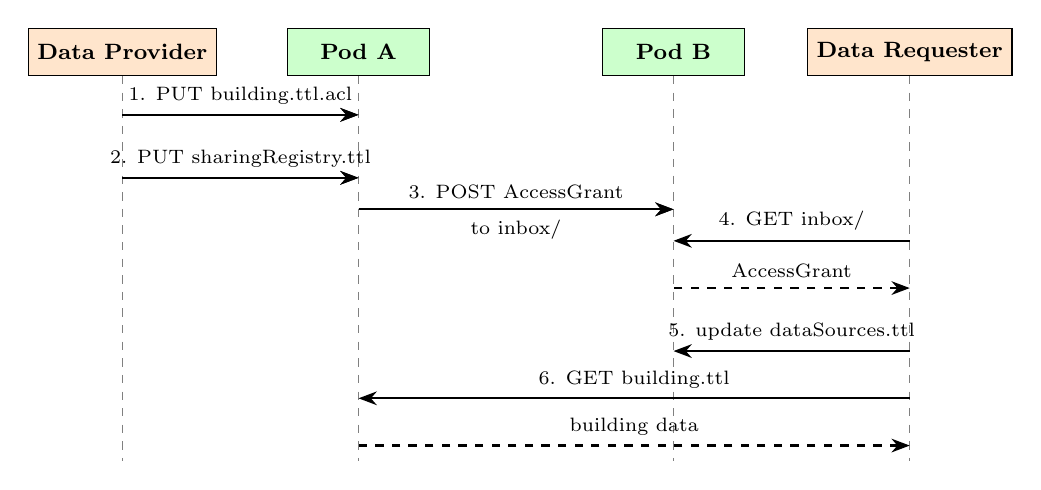
\begin{tikzpicture}[
    % Styles
    entity/.style={
        rectangle,
        draw=black,
        fill=#1,
        minimum width=1.8cm,
        minimum height=0.6cm,
        align=center,
        font=\footnotesize\bfseries
    },
    entity/.default=orange!20,
    lifeline/.style={
        dashed,
        gray
    },
    msg/.style={
        -Stealth,
        thick
    },
    msgback/.style={
        Stealth-,
        thick,
        dashed
    }
]

% Entities (participants)
\node[entity] (provider) at (0, 0) {Data Provider};
\node[entity=green!20] (podA) at (3, 0) {Pod A};
\node[entity=green!20] (podB) at (7, 0) {Pod B};
\node[entity] (requester) at (10, 0) {Data Requester};

% Lifelines
\draw[lifeline] (provider.south) -- (0, -5.2);
\draw[lifeline] (podA.south) -- (3, -5.2);
\draw[lifeline] (podB.south) -- (7, -5.2);
\draw[lifeline] (requester.south) -- (10, -5.2);

% Messages - Sharing flow
\draw[msg] (0, -0.8) -- node[above, font=\scriptsize] {1. PUT building.ttl.acl} (3, -0.8);
\draw[msg] (0, -0.8) -- node[below, font=\scriptsize] {} (3, -0.8);

\draw[msg] (0, -1.6) -- node[above, font=\scriptsize] {2. PUT sharingRegistry.ttl} (3, -1.6);
\draw[msg] (0, -1.6) -- node[below, font=\scriptsize] {} (3, -1.6);

\draw[msg] (3, -2) -- node[above, font=\scriptsize] {3. POST AccessGrant} (7, -2);
\draw[msg] (3, -2) -- node[below, font=\scriptsize] {to inbox/} (7, -2);

% Messages - Requester processing
\draw[msg] (10, -2.4) -- node[above, font=\scriptsize] {4. GET inbox/} (7, -2.4);
\draw[msgback] (10, -3) -- node[above, font=\scriptsize] {AccessGrant} (7, -3);

\draw[msg] (10, -3.8) -- node[above, font=\scriptsize] {5. update dataSources.ttl} (7, -3.8);

% Messages - Data access
\draw[msg] (10, -4.4) -- node[above, font=\scriptsize] {6. GET building.ttl} (3, -4.4);
\draw[msgback] (10, -5) -- node[above, font=\scriptsize] {building data} (3, -5);

% Annotations
% \draw[decorate, decoration={brace, amplitude=5pt, mirror}] (-0.5, -0.6) -- (-0.5, -2.4) node[midway, left=6pt, font=\scriptsize, align=right] {Granting\\access};
% \draw[decorate, decoration={brace, amplitude=5pt}] (10.5, -2) -- (10.5, -3.8) node[midway, right=6pt, font=\scriptsize, align=left] {Processing\\notification};

\end{tikzpicture}
\caption{Sequence diagram of the data sharing process: the Data Provider grants access by updating the ACL and sending a notification; the Data Requester processes the notification and can then fetch the shared data.}
\label{fig:sharing-process}
\end{figure}

Revocation removes the recipient's authorization from the ACL; subsequent access attempts return HTTP~403, prompting automatic cleanup of the recipient's \mintinline{text}{dataSources.ttl}.

\subsection{Sharing Aggregated Data}

While sharing individual building data enables direct collaboration between pairs such as the FM and tenant, the investor -- BSP scenario (\cref{tbl:invroom}) demonstrates a different need: computing aggregated statistics across multiple properties without exposing the individual buildings.
The GRANERGIZE WebApp addresses this through aggregated views -- snapshots containing only computed values.

An aggregated view is defined by three parameters: a set of source buildings, an aggregation function (\mintinline{text}{sum}, \mintinline{text}{average}, \mintinline{text}{minimum}, or \mintinline{text}{maximum}), and a selection of energy metrics.
\cref{fig:create-agg-view} shows the user interface for creating a view, and \cref{lst:view-definition} shows the resulting Turtle definition stored in the owner's Pod.
Note, that the view definition itself -- including the source building URIs -- is never shared.
Only the computed snapshot, containing aggregated values without provenance information, is made accessible to recipients.

When the owner creates or refreshes a view, the application fetches energy data from each source building, applies the selected aggregation function, and stores the result as a separate snapshot file.
\begin{figure}[t]
\noindent\begin{minipage}[t]{0.38\textwidth}
\vspace{0pt}
\centering
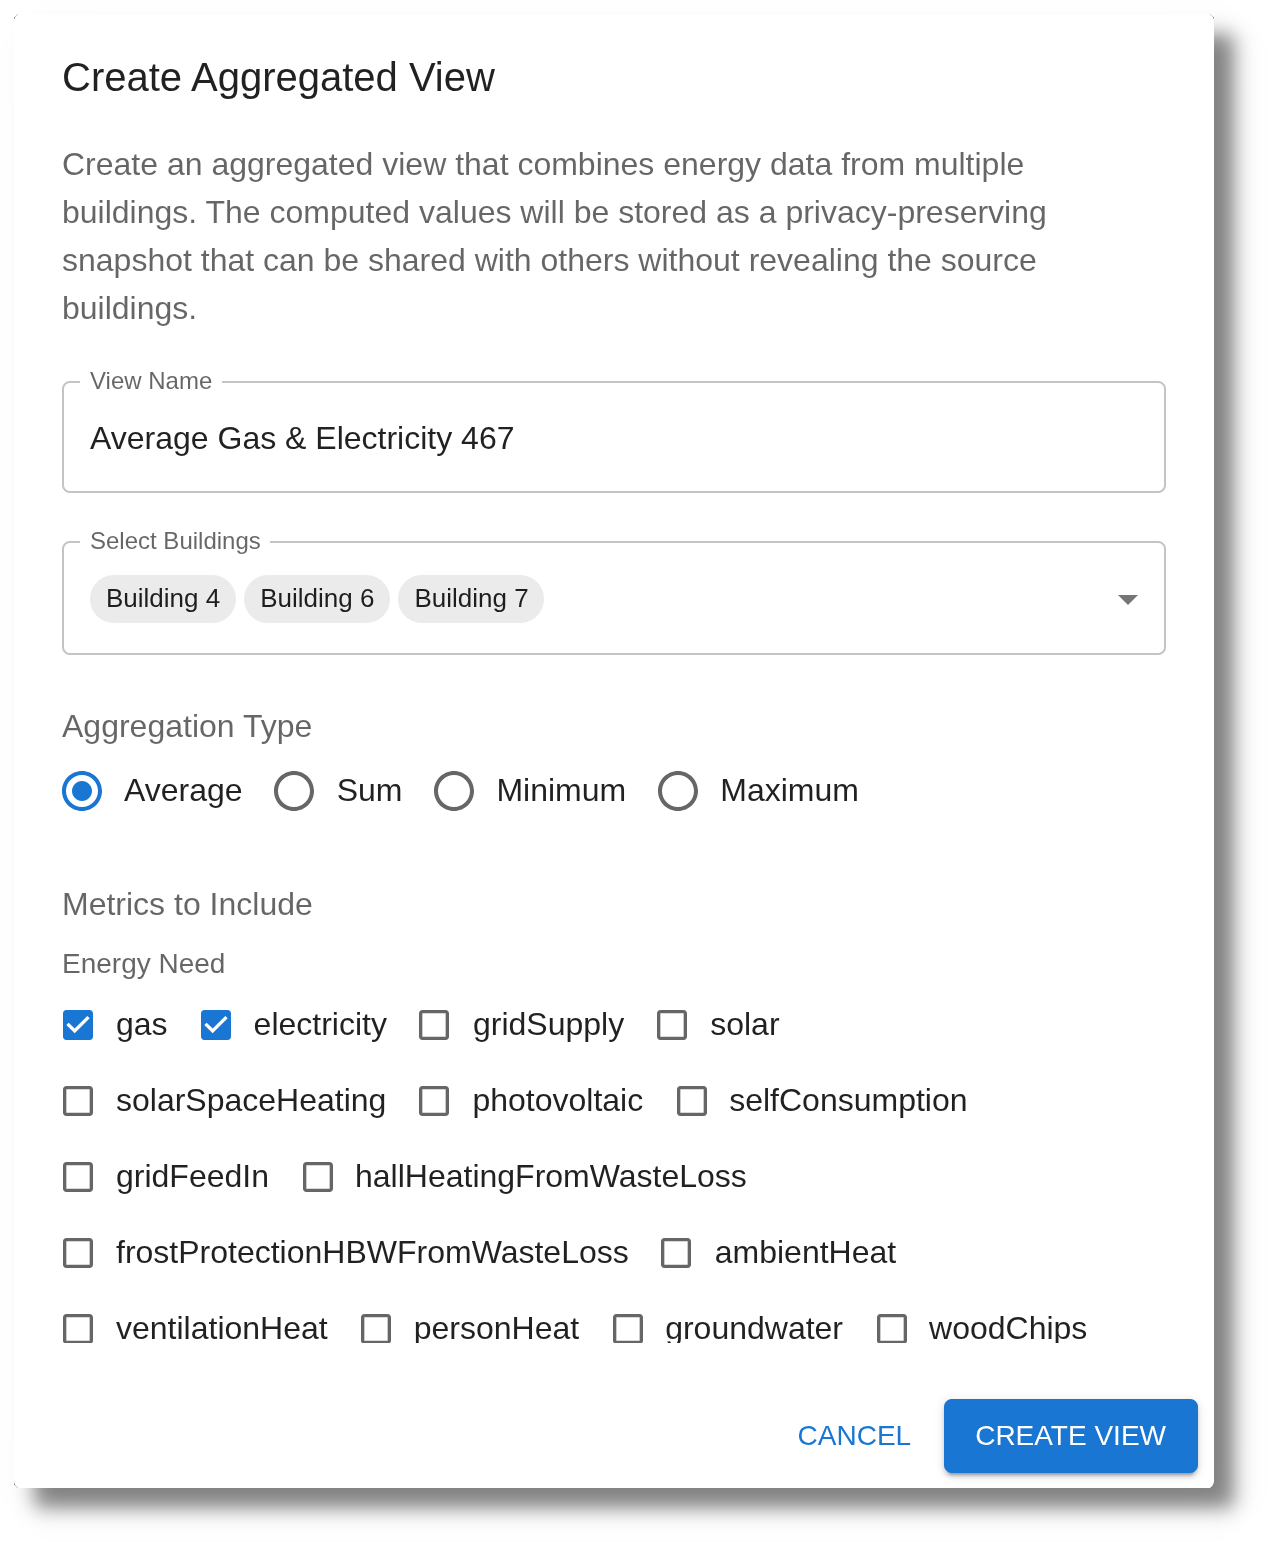
\includegraphics[width=\textwidth]{create-agg-view.png}
\captionof{figure}{Create Aggregated View Dialog}
\label{fig:create-agg-view}
\end{minipage}\hfill%
\begin{minipage}[t]{0.6\textwidth}
\vspace{0pt}
\centering
\begin{minted}[linenos, frame=lines, fontsize=\footnotesize, breaklines]{turtle}
<#view-1770048602886-f5n4sea> a gra:AggregatedViewDefinition ;
  gra:viewId "view-1770048602886-f5n4sea" ;
  gra:viewName "Average Gas and Electricity 467" ;
  gra:aggregationType "average" ;
  gra:createdAt "2026-02-02T16:10:02.886Z"^^xsd:dateTime ;
  gra:includesBuilding <../private/granergize/buildings/4.ttl>,
    <../private/granergize/buildings/2.ttl>,
    <../private/granergize/buildings/6.ttl> ;
  gra:includesMetric "gas", "electricity" ;
  gra:lastComputedAt "2026-02-02T16:10:04.064Z"^^xsd:dateTime .
\end{minted}
\captionof{listing}{View Definition Example}
\label{lst:view-definition}
\end{minipage}
% \noindent\begin{minipage}[t]{0.46\textwidth}
% \vspace{0pt}
% \centering
% 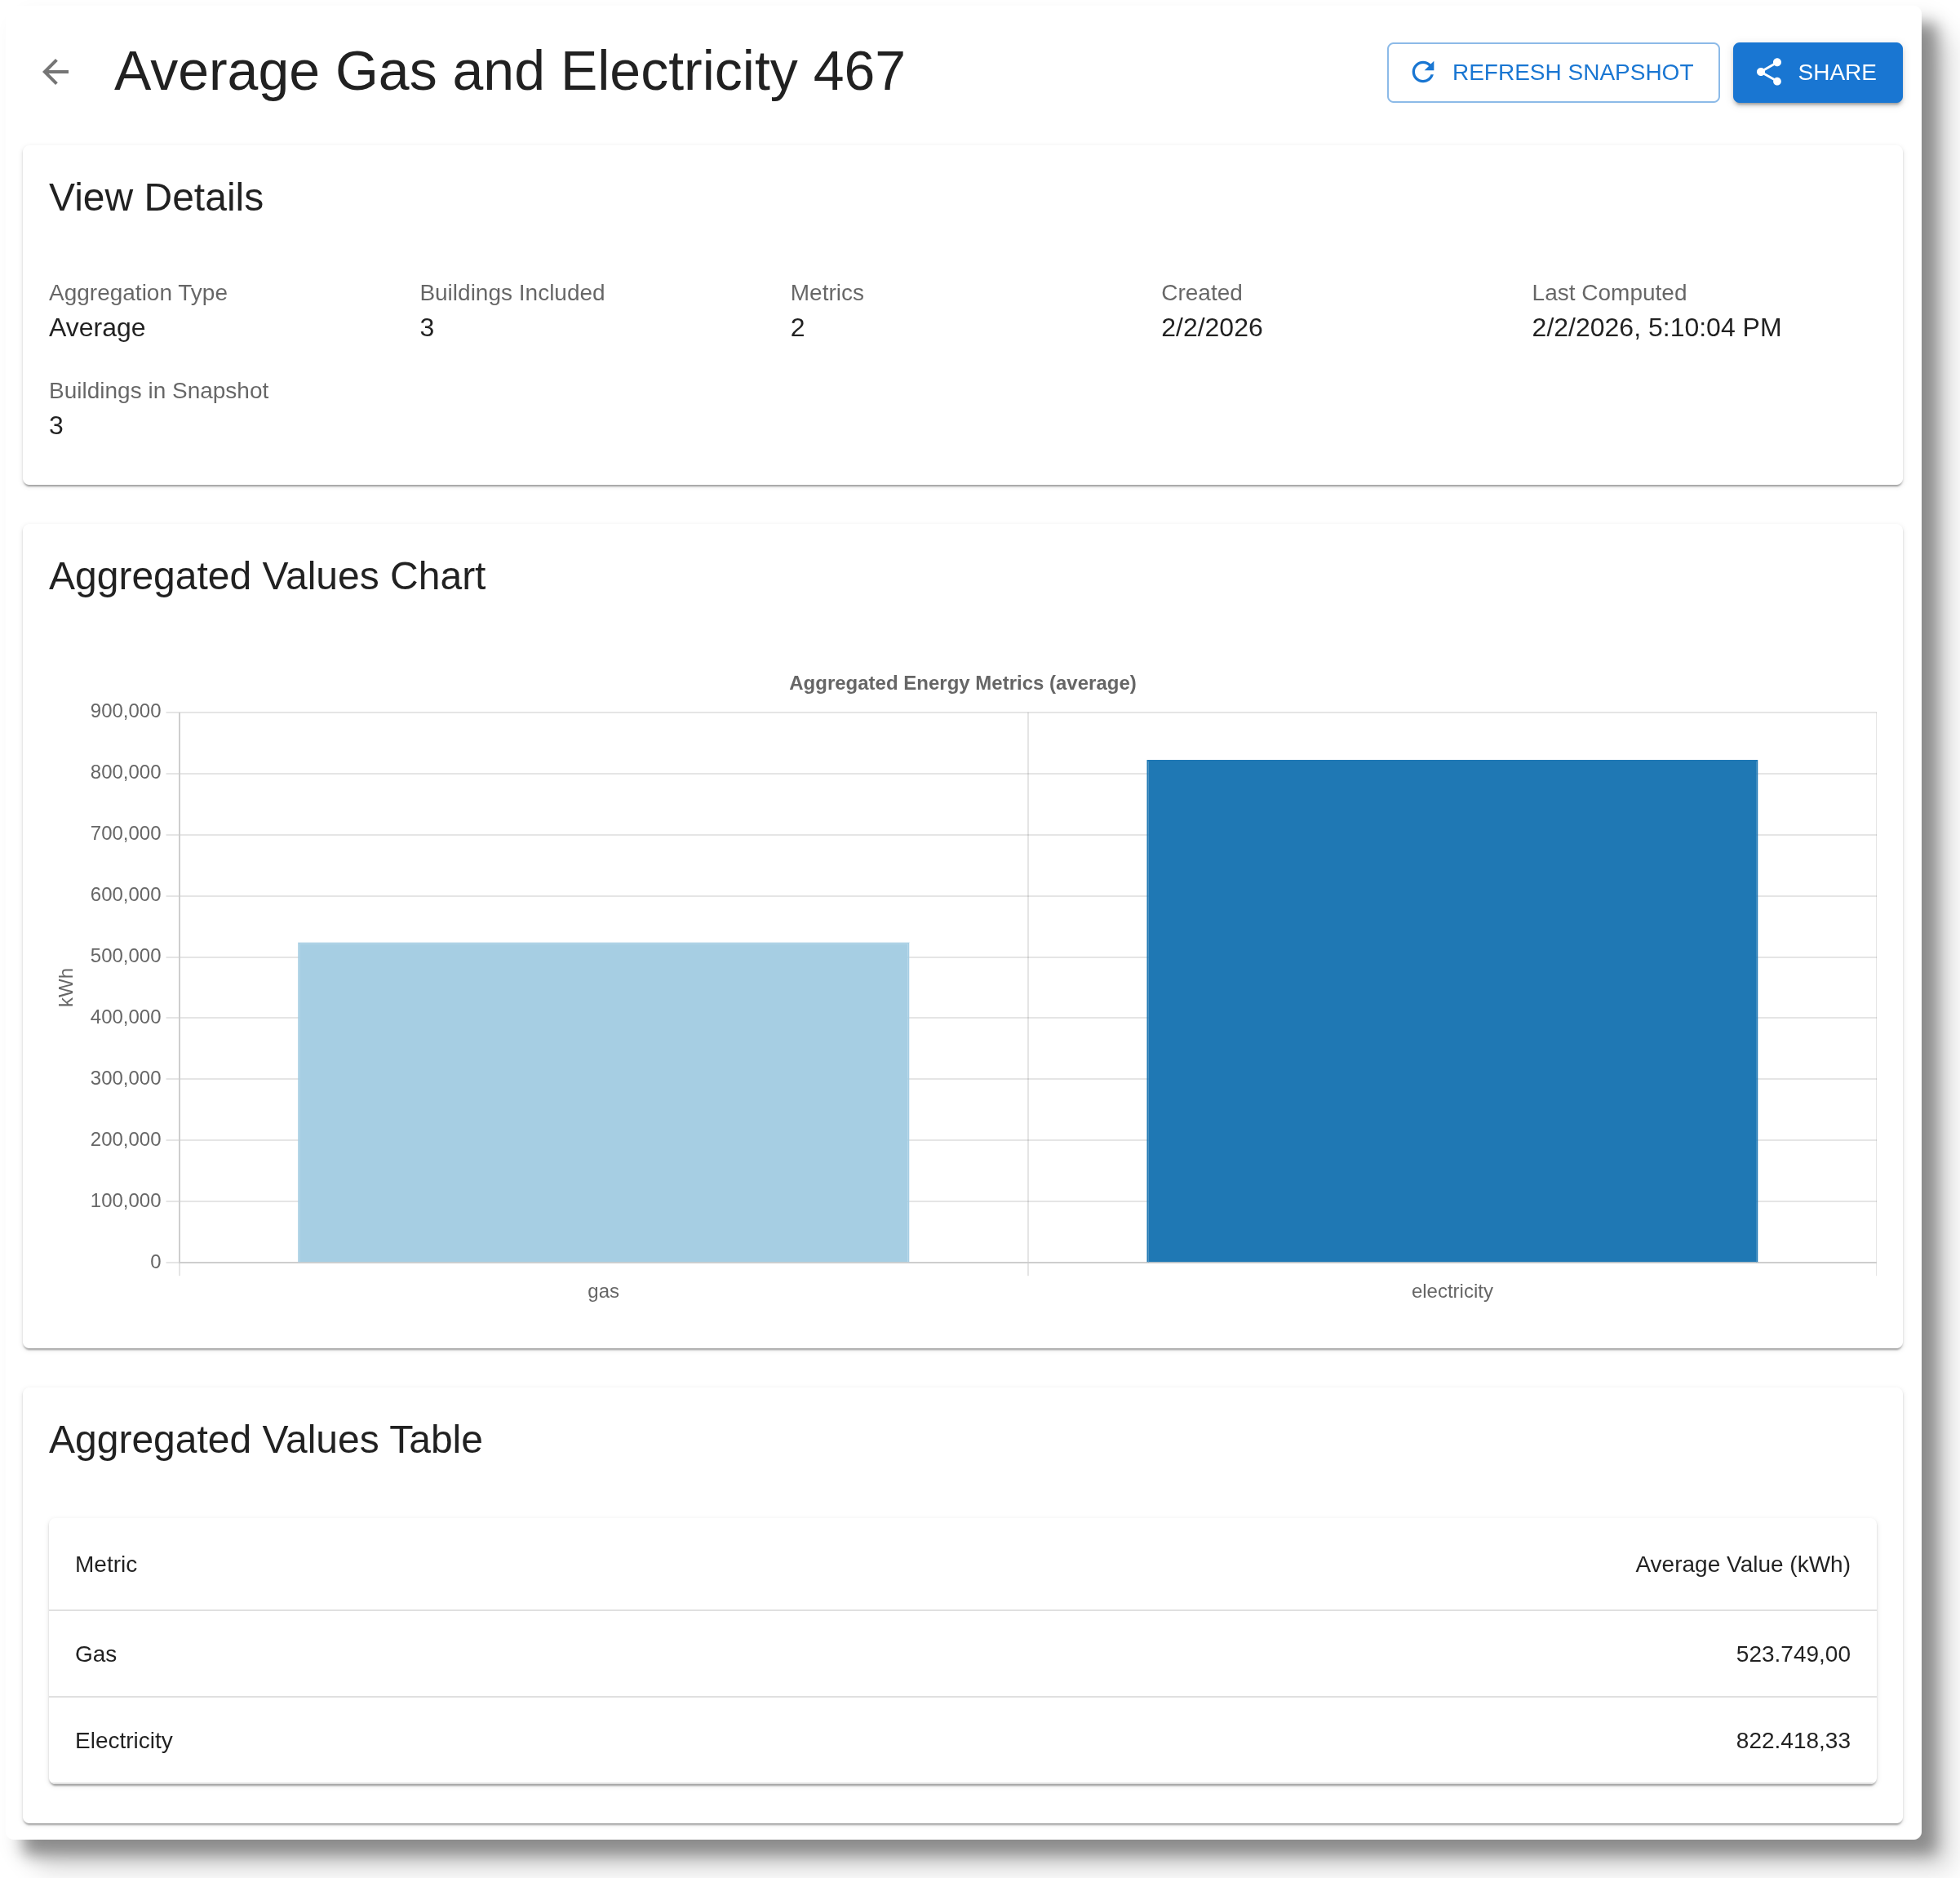
\includegraphics[width=\textwidth]{create-agg-data.png}
% \captionof{figure}{Create Aggregated View Dialog}
% \label{fig:agg-data}
% \bigskip
% \end{minipage}\hfill%
% \begin{minipage}[t]{0.53\textwidth}
% \vspace{0pt}
% \centering
% \begin{minted}[linenos, frame=lines, fontsize=\footnotesize, breaklines]{turtle}
% <#snapshot> a gra:AggregatedViewSnapshot ;
%   gra:viewId "view-1770048602886-f5n4sea" ;
%   gra:viewName "Average Gas and Electricity 467" ;
%   gra:aggregationType "average" ;
%   gra:computedAt "2026-02-02T16:10:04.064Z"^^xsd:dateTime ;
%   gra:buildingCount 3 ;
%   gra:includesMetric "gas", "electricity" ;
%   gra:gasValue 523749.00 ;
%   gra:electricityValue 822418.33 .
% \end{minted}
% \captionof{listing}{View Definition Example}
% \label{lst:view-snapshot}
% \bigskip
% \end{minipage}
% \Cref{fig:agg-data} shows an example of such a snapshot for the view defined in \cref{lst:view-definition}.
\end{figure}

Sharing and revoking access to aggregated views follows the same WAC-based pattern as individual buildings.
Because snapshots are materialized, shared values reflect the state at the time of last refresh; owners can update by triggering a manual recomputation.

\section{Conclusion}

Energy consumption data in the logistics sector remains fragmented across organizational boundaries, preventing effective benchmarking and collaboration.
Centralized platforms require stakeholders to surrender data control, conflicting with privacy requirements and competitive interests.

This paper introduces the concept of Data Rooms -- a structured process for stakeholders to identify and formalize data sharing requirements, establishing trust and enabling partner discovery before any data is exchanged. Additionally, we present the GRANERGIZE WebApp, a Solid-based application that addresses these challenges through decentralized data sharing while preserving data sovereignty.
The implementation demonstrates how WAC for fine-grained permissions and the INTEROP specification for access notifications can solve real-world data-sharing problems without centralized data custody.
The aggregated views feature extends the sharing model to support statistical summaries without exposing individual building details.

A key area for future development is integrating Data Room functionality directly into the WebApp, enabling stakeholders to discover potential partners, and manage data sharing agreements within the application.
Additional future work includes integrating automated access request workflows, data integration pipelines, and supporting additional aggregation functions such as weighted averages based on building size.
We also plan to evaluate the system's usability with logistics stakeholders in a field study.


\section{Acknowledgements}
We acknowledge funding from the German Federal Ministry for Economic Affairs and Energy (FKZ 01IF23286N).

%%
%% Define the bibliography file to be used
\bibliography{references}

\end{document}

%%D
%% End of file

